\section{二次函数实际问题}


\subsection{有关图形}

有关图形的问题比较多样.重点在于理解问题,一般来说需要一步一步地将几个量的表达式推导出来(利用数量关系、利用几何关系).有些题目的数量关系比较复杂,捋清楚关系才能得到表达式,同时不能忽略自变量的取值范围.

本节给不同的题目进行分类,看似复杂实际上都是一样的底层逻辑.


\subsubsection*{围墙}


\begin{wrapfigure}{r}{3cm}
    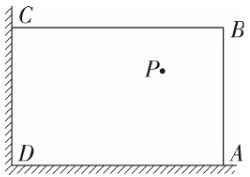
\includegraphics[width=1\linewidth]{figure/p1.png}
    \caption{}
    \label{fig:p1}
\end{wrapfigure}

\exas{
如图\ref{fig:p1},某劳动小组借助一个直角墙角围成一个矩形劳动基地 $ABCD$,墙角两边 $DC$ 和 $DA$ 足够长,用总长 $28\ \text{m}$ 的篱笆围成另外两边 $AB$ 和 $BC$,有下列结论:

\begin{enumerate}
    \item 当 $AB$ 的长是 $10\ \text{m}$ 时,劳动基地 $ABCD$ 的面积是 $180\ \text{m}^2$;
    \item $AB$ 的长有两个不同的值满足劳动基地 $ABCD$ 的面积为 $192\ \text{m}^2$;
    \item 点 $P$ 处有一棵树(树的粗细忽略不计),它到墙 $DC$ 的距离是 $12\ \text{m}$,到墙 $DA$ 的距离是 $8\ \text{m}$,如果这棵树需在劳动基地内部(包括边界),那么劳动基地面积的最大值是 $196\ \text{m}^2$,最小值是 $160\ \text{m}^2$.
\end{enumerate}

其中,正确结论的个数是(\hspace{3.5em})

\begin{enumerate*}[label=\Alph*.]
    \item 0 \hspace{3em}
    \item 1 \hspace{3em}
    \item 2 \hspace{3em}
    \item 3
\end{enumerate*}
}{
分析:(1)先要知道边\(AB\)与面积的关系,所以设\(AB\)为自变量\(x\),因为总长为28,所以\(BC\)的长为\((28-x)\),所以\(y=x(28-x)\),将\(10\)代入,求得结果确实是180所以正确.(2)前面得出了\(y=x(28-x)\),这里问边长\(AB\)与面积的关系所以继续使用\(y=x(28-x)\)表达,接着代入\(192\)到函数,思路一:计算判别式,看\(x(28-x)=0\)与\(y=192\)是否有两个交点,思路二:因式分解解方程,如果结果有两个,则确实有两个不同的值满足条件.经过计算(2)正确.(3)由题意可知\(\begin{cases}
x>8\\
28-x>12
\end{cases}\)解得\(8\le x \le 16\)是关于\(x\)的区间,将\(x=8\)和\(x=16\)分别代入函数\(y=x(28-x)\),分别得到160和192,所以函数的最小值应该是160,因为函数开口向下,所以顶点纵座标是函数最大值,将函数化为顶点式得\(y=-(x-14)^2+196\),所以最大值为196.以上三个选项都正确,故选\(D\)
}


\begin{wrapfigure}{r}{3cm}
    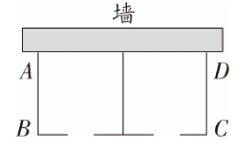
\includegraphics[width=1\linewidth]{figure/p2.png}
    \caption{}
    \label{fig:p2}
\end{wrapfigure}

\subsubsection*{分割}

\exas{
如图\ref{fig:p2},园林部门计划在某公园建一个长方形苗圃 $ABCD$,苗圃的一面靠墙(墙最大可用长度为 $14\ \text{m}$),另三边用木栏围成,中间也用垂直于墙的木栏隔开,分成两个区域,并各留 $2\ \text{m}$ 宽的门(门不用木栏),若建成后所用木栏总长为 $32\ \text{m}$,则长方形 $ABCD$ 的最大面积为(\hspace{3.5em})
\begin{enumerate*}[label=\Alph*.]
    \item $\dfrac{22}{3}\ \text{m}^2$ \hspace{3em}
    \item $108\ \text{m}^2$ \hspace{3em}
    \item $\dfrac{318}{3}\ \text{m}^2$ \hspace{3em}
    \item $\dfrac{308}{3}\ \text{m}^2$
\end{enumerate*}
}{
分析:要求面积最值,实际上是要先求边与面积的关系,题目没有给出具体边长,所以这里需要设完整的两条边来求,可以选择先设\(AB,DC\)或\(AD\),这里示例设\(AB\)为\(x\),要求面积还需要另外一条完整的边,因为留了2m的门(注意这里有两个门是4m)、墙的一面没有用木栏围住、中间用长\(x\)的木栏隔开(平行线间的距离处处相等),设中间的隔板为\(MN\),所以加上\(32+2\times2=36\)的长是\(AB+BC+CD+MN=36\),代入\(x\)得\(3x+BC=36\),所以\(BC=AD=36-3x\),这里题目还要求墙的最长为\(14\)所以\(36-3x\le14\)解得\(x\ge\dfrac{22}{3}\).表示出长和宽就能表示\(ABCD\)的面积为\(y=x(34-x)\ (x\ge\dfrac{20}{3})\),此时就将面积最值问题转化为区间最值问题(注意这里的区间范围不能使用顶点式求最值).解得最大值为\(\dfrac{308}{3}\), 故\(D\)正确.
}

\begin{wrapfigure}{r}{3cm}

    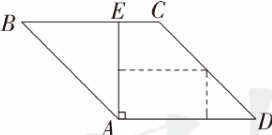
\includegraphics[width=1\linewidth]{figure/p3.png}
    \caption{}
    \label{fig:p3}
    
\end{wrapfigure}

\exas{
如图\ref{fig:p3},是一块菱形新型平面材料 \(ABCD\),
\(\angle BAD = 135^\circ\),\(AB = 50\ \text{cm}\),点 \(E\) 在 \(BC\) 上,且
\(EA \perp AD\),先沿着 \(AE\) 切开材料,然后在四边形 \(ADCE\) 内切割出一块矩形,且矩形相邻两条边分别落在 \(AD\)、\(AE\) 上,一个顶点落在 \(CD\) 边上.设边 \(AE\) 上矩形的边长为 \(x\ \text{cm}\),矩形的面积为 \(y\ \text{cm}^2\),有下列结论:

\begin{enumerate}
    \item \(y\) 与 \(x\) 之间的函数解析式为 \(y = -x^2 + 50x \quad (0 < x \leq 25\sqrt{2})\);
    \item 当 \(x = 10\) 时,切割出矩形后,四边形 \(AECD\) 剩余的面积为 \((1250\sqrt{2} - 625)\ \text{cm}^2\);
    \item 若切割出的矩形材料用于某种生产时,售价为 \(1.5\ \text{元}/\text{cm}^2\),则当 \(x = 25\) 时,出售此块矩形材料的总价最大,最大值为 \(937.5\ \text{元}\).
\end{enumerate}

其中,正确结论的个数是\(\underline{\hspace{3em}}\).

\begin{enumerate*}[label=\Alph*.]
    \item 0 \hspace{3em}
    \item 1 \hspace{3em}
    \item 2 \hspace{3em}
    \item 3
\end{enumerate*}

}{
\begin{wrapfigure}{r}{3cm}
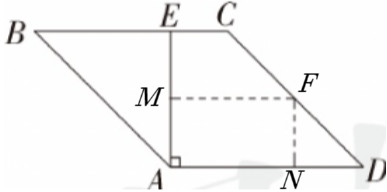
\includegraphics[width=1\linewidth]{figure/p3-1.png}
    \label{fig:p3_1}
    \caption{}
\end{wrapfigure}
分析:在正式分析之前需要先将题目所给得信息正利好,已知菱形中一个角\(\angle BAD=135^\circ\),推导能得出\(\angle B= \angle D=45^\circ\),因为\(AB=50cm\)所以其他三条边也是\(50cm\).(1)要验证解析式是否正确,实际上是要用边长与面积的关系构造函数,如图设点\(M,F,N\),则\(AM=x\),还要注意\(x\)所在的范围,因为四边形\(ABCD\)是矩形,所以\(A,B,C,D\)四点不共线,也就是说\(M\)不与\(A\)重合,\(F,N,D\)都不重合,所以\(x>0\),因为切割的矩形在菱形内,所以\(MA\le EA\),根据已知信息可以推导\(EA=25\sqrt{2}\),综合起来\(0<x\le25\sqrt{2}\).表示出\(MA\)后就要表示矩形的另外一边,这里选择表示\(AN\)比较方便,因为推导可得\(ND=FN=x\),又\(AD=50cm\),所以\(AN=AD-ND=50-x(cm)\),所以切割矩形面积的函数\(y=x(50-x)\quad(0<x\le25\sqrt{2})\),整理为一般形式\(y=-x^2+50x\quad(0<x\le25\sqrt{2})\),故(1)正确.

(2)要求证剩余面积,实际上是问切割矩形的面积与剩余面积的关系:剩余面积=四边形\(AECD\)面积-切割矩形面积.以此构造函数,最后代入\(x=10\) ,得到结果\(1250\sqrt{2}-1025\).故(2)错误.

(3)要求售价最大,实际上是问单价与切割面积的关系,以此构造函数\(w=1.5(-x^2+50x)\quad (0<x\le25\sqrt{2})\),将其整理为一般形式\(w=-\dfrac{3}{2}x^2+75\quad (0<x\le25\sqrt{2})\) 因为该函数开口向下所以有最大值,将其整理为顶点式得到\(w=-1.5(x-25)+937.5\) ,因此当\(x=25\)时确实取最大值,且最大值确实为\(937.5\) ,故(3)正确

综上,有两个结论正确,故选\(C\)
}

\subsubsection*{动点}

\begin{wrapfigure}{r}{3cm}
\vspace{-1cm}
    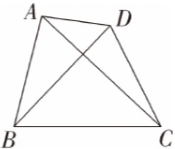
\includegraphics[width=1\linewidth]{figure/p4.png}
    \caption{}
    \label{fig:p4}
\end{wrapfigure}

\exas{
如图\ref{fig:p4},某公园的示意图是对角线互相垂直的四边形 \(ABCD\),已知 \(AC+BD=160\) 米,则该四边形公园的最大面积为\underline{\hspace{3.5em}}平方米.

}{
要求面积最大值,首先要列出面积的表达式,观察图形,可以将该四边形分为两个三角形,这里以\(\triangle ABC\)与\(\triangle ADC\)为例,设\(AC\)与\(BD\)相交于点\(M\),就能顺利构造函数\(s=S_{\triangle ABC}+S_{\triangle ADC}=\dfrac{1}{2}AC \cdot BM + \dfrac{1}{2}AC \cdot DM\),整理得\(s=\dfrac{1}{2}AC \cdot BD\).接下来就需要表示\(AC\)和\(BD\) .根据\(AC+BD=160\),设\(AC\)为\(x\)则\(BD\)为\(160-x\),所以\(s=\dfrac{1}{2}x(160-x)\)整理得\(s=-\dfrac{1}{2}x^2+80x\).因为该函数开口向下,所以有最大值,将其写为顶点式,计算得最最大值为\(3200m^2\) ,故四边形公园的最大面积为\(3200m^2\)



}

\begin{wrapfigure}{r}{3cm}
\vspace{-1.8cm}
    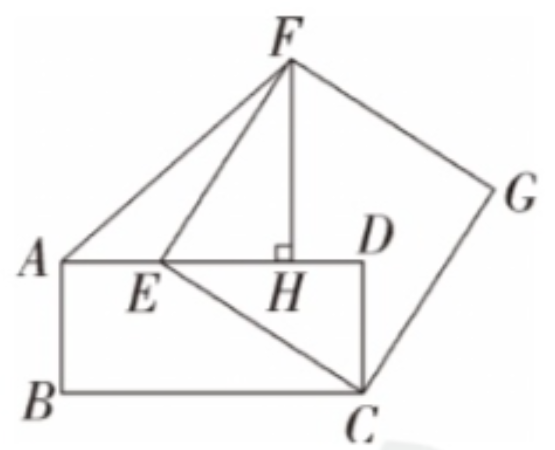
\includegraphics[width=1\linewidth]{figure/p5.png}
    \caption{}
    \label{fig:p5}
\end{wrapfigure}


\begin{example}
    如图\ref{fig:p5},在矩形 \(ABCD\) 中,\(AD=4\),\(E\) 是 \(AD\) 边上的动点,连接 \(CE\),以 \(CE\) 为边向右上方作正方形 \(CEFG\),过点 \(F\) 作 \(FH \perp AD\),垂足为点 \(H\),连接 \(AF\).在整个变化过程中,\(\triangle AEF\) 面积的最大值是\underline{\hspace{3.5em}}.
\end{example}

\begin{wrapfigure}{r}{3cm}
    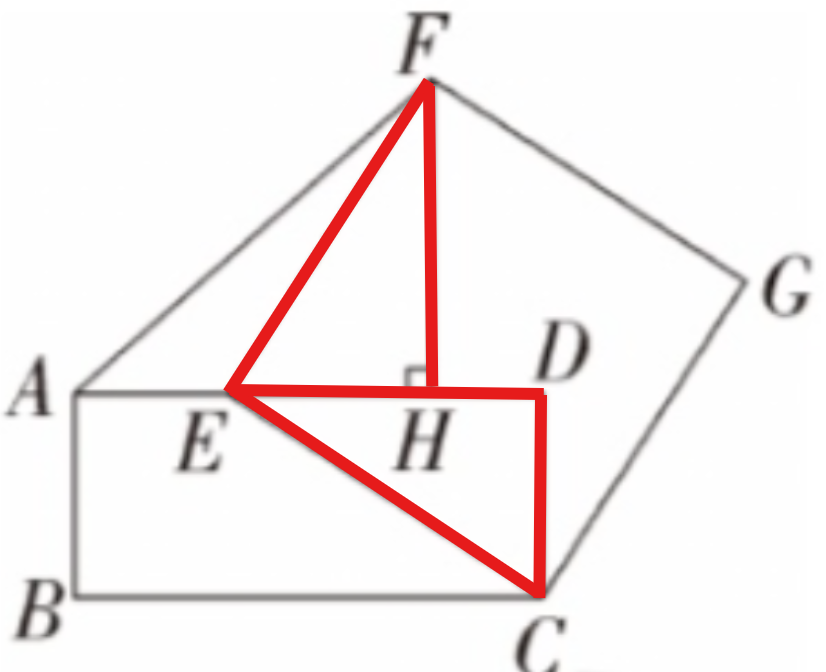
\includegraphics[width=1\linewidth]{figure/p5-1.png}
    \caption{}
    \label{fig:p5_1}
\end{wrapfigure}

\begin{solution}
分析:首先构造\(\triangle AEF\)面积的函数\(s=\dfrac{1}{2}AE\cdot FH\),接下来就要建立\(AE\)和\(FH\)的联系.观察图形,可知\(AE=AD-ED=4-ED\),就将\(AE\)转化为先求\(ED\),观察图形(如图\ref{fig:p5_1})可以发现\(ED\)与\(FH\)存在联系,通过“一线三垂直”推导可得\(ED=FH\),所以设\(FH=x\),则\(AE=4-x\),注意\(x\)的取值,因为\(E\)是\(AD\)上的动点,所以\(0\le4-x\le4\),化简得\(0\le x\le 4\),代入函数解析式得\(s=\dfrac{1}{2}x(4-x)\quad(0\le x\le 4)\),将其写为顶点式,当\(x=2\)时,函数\(s\)取得最大值是2,且在区间内是最大值符合题意.故\(\triangle AEF\) 面积的最大值是2

\end{solution}


\subsection{有关商品销售}



\exas{
某商场要经营一种新上市的文具,进价为10元/件.试营销阶段发现:当销售单价为20元时,每天的销售量是200件;销售单价为30元时,每天的销售量是100件.其中每天的销售量是售价的一次函数.

\begin{enumerate}[label=(\arabic*)]
    \item 求这种文具每天的销售量 $y$ (件) 与销售单价 $x$ (元) 之间的函数解析式;
    
    \item 销售单价为多少元时,该文具每天的销售利润最大?
\end{enumerate}
}{
分析:(1)已知单售价为自变量,销售量为因变量,由题意知他们的关系式是一次函数,所以设\(y=kx+b\),代入题目所给数据求出解析式为\(y=-10x+400\)
(2)首先明确要求销售利润与单价的关系式,要知道每日销售利润=单品利润\(\times\)每日总销售量,单品利润=单品售价-单品进价,那么由题意得单品利润为\(x-10\) ,每日销售量为\(-10x+400\),即可构造函数\(w=(x-10)(-10x+400)\) ,整理得\(w=-10x^2+500x-4000\),将其写为顶点式,得当\(x=25\)时,函数取得最大值2250 .

}


\begin{wrapfigure}{r}{6cm}
    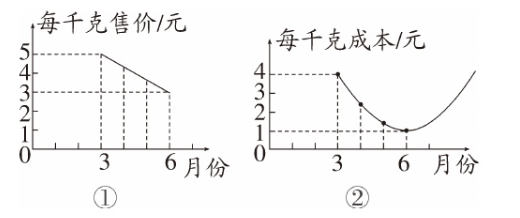
\includegraphics[width=1\linewidth]{figure/p7.png}
    \caption{}
    \label{fig:p7}
\end{wrapfigure}

\exas{
某种蔬菜的销售单价与销售月份之间的关系如图\textcircled{1}所示,成本与销售月份之间的关系如图\textcircled{2}所示(图\textcircled{1}的图象是线段,图\textcircled{2}的图象是抛物线).\underline{\hspace{1cm}}月出售这种蔬菜,每千克的收益最大.(收益=售价-成本)
}{
分析:题目给出售价与月份的关系和成本与月份的关系,如果知道售价的解析式和成本的解析式,代入收益=售价-成本就能表示出收益的解析式,写成顶点式的形式就能取得最值.由题意和图像可以知道售价和成本都受月份影响,所以将月份作为自变量\(x\),售价和成本分别为两个函数\(y_1,y_2\),图中给出\(y_1,y_2\)上一些点的坐标,分别求出\(y_1,y_2\)的解析式,设收益为\(w\)则\(w=y_1-y_2\),再对\(w\)配方取得最值.最后注意题目问的是月份,不要写成最值.
}





\subsection{有关抛物线形状}


\begin{wrapfigure}{r}{6cm}
    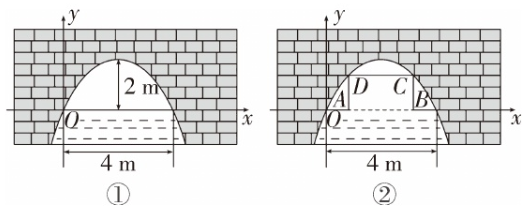
\includegraphics[width=1\linewidth]{figure/p8.png}
    \caption{}
    \label{fig:p8}
\end{wrapfigure}

\exas{
如图\ref{fig:p8}为抛物线形拱桥平面示意图,拱顶离水面 2 m,水面宽 4 m.以现有水平面的水平直线为 \( x \) 轴,与抛物线形拱桥左边交点为原点建立平面直角坐标系.

\begin{enumerate}
    \item 求此抛物线解析式.
    
    \item 如图\textcircled{1},若水面下降1 m,水面宽度增加多少米?
    
    \item 如图\textcircled{2},为保证行船安全,在汛期来临之前,管理部门需要用一定长度的钢板搭建一个可调节大小的矩形"安全架",露出水平面部分为 \( AD-DC-CB \),使点 \( C, D \) 在抛物线上,点 \( A, B \) 为露出水面的端点,若确保点 \( A, B \) 的间距不少于3 m,求 \( AD-DC-CB \) 的最大长度.
\end{enumerate}
}{}

\begin{wrapfigure}{r}{6cm}
    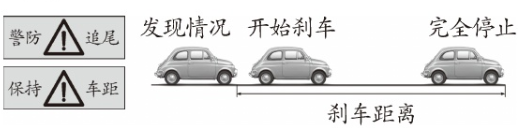
\includegraphics[width=1\linewidth]{figure/p9.png}
    \caption{}
    \label{fig:p9}
\end{wrapfigure}

\exas{
随着时代的进步,我国交通出行结构发生根本性变化,汽车出行成为交通常态.某数学兴趣小组观察校门口的汽车发现,很多车尾部贴上了保持车距的贴纸.小组成员产生了一个困惑——"保持怎样的车距才能保障道路安全?"为解决这一困惑,小组成员分工开展活动:
成员小梧查阅某型号汽车官网数据得到汽车行驶速度 $x$ (m/s) 与刹车距离 $y$ (m) 的关系如表(刹车距离:从发现前方道路有异常情况到车辆完全停止所行驶的距离.)

\begin{table}[h]
\centering
\caption{某型号汽车行驶速度 $x$(m/s) 与刹车距离 $y$(m) 的关系}
\begin{tabular}{|c|c|c|c|c|c|c|c|}
\hline
行驶速度 $x$/(m/s) & 0 & 5 & 10 & 15 & 20 & 25 & 30 \\
\hline
刹车距离 $y$/m & 0 & 3.25 & 9 & 17.25 & 28 & 41.25 & 57 \\
\hline
\end{tabular}
\end{table}

\begin{itemize}
    \item 任务1:小梧认为该型号汽车的行驶速度 $x$ (m/s) 与刹车距离 $y$ (m) 之间存在函数关系,请你协助小梧求出该函数解析式.
    \item 任务2:成员小杭发现小区门口路段限速60 km/h.请你帮小杭计算,如果该型号汽车以最高限速60 km/h行驶,至少保持多少车距才能保障道路安全?
    \item 任务3:实际驾驶过程中,驾驶员难以预估前车的距离,且难以实时计算不同行驶速度对应的安全距离,是否存在简单、实用且能维持适当安全距离的方案?小组成员带着困惑与陈老师进行交流,陈老师分享了他保持车距常用的方案"2秒定律"——跟车行驶时设定一个参照物,前车超越参照物后,后车如果在两秒内到达该参照物,说明与前车的距离不足,反之距离充足.
\end{itemize}
}{}